\chapter{Empirical prediction results}

On \textbf{ETTh1}~\ref{tab:etth-metrics}, \textsc{CSDI} attains the lowest RMSE/MAE/CRPS/CRPS(sum) which might be due to it's harder transformer backbone and more broad feature-time encoder; \textbf{FITS} is consistently second-best, improving over \textsc{DiffusionTS} and \textsc{FMTS} on both point-error and distributional metrics.

\begin{table}[ht]
\centering
\caption{ETTh Dataframe metrics}
\label{tab:etth-metrics}
\begin{tabular}{lrrrrr}
\toprule
Metric & {CSDI} & {DiffusionTS} & {FMTS} & {FMTS (first diff.)} & {\textbf{FITS (our)}} \\
\midrule
RMSE        & 3.023 & 4.057 & 4.113 & 4.603 & 3.835 \\
MAE         & 1.619 & 2.377 & 2.445 & 2.444 & 2.129 \\
CRPS        & 0.245 & 0.401 & 0.426 & 0.423 & 0.366 \\
CRPS (sum)  & 0.237 & 0.317 & 0.348 & 0.415 & 0.323 \\
\bottomrule
\end{tabular}
\\[2pt]
{\footnotesize Note: Lower is better for all metrics; CRPS/CRPS(sum) evaluate probabilistic calibration and sharpness over the forecast horizon on ETTh1.}
\end{table}

On \textbf{Solar}~\ref{tab:solar-metrics}, \textbf{FITS} is best on all metrics, with the largest margin on CRPS(sum), indicating improved horizon-level probabilistic accuracy; \textsc{FMTS (first diff.)} improves over \textsc{FMTS} on RMSE/MAE but remains behind \textbf{FITS}, and \textsc{CSDI} underperforms on this dataset.

\begin{table}[ht]
\centering
\caption{Solar Dataframe metrics}
\label{tab:solar-metrics}
\begin{tabular}{lrrrrr}
\toprule
Metric & {CSDI} & {DiffusionTS} & {FMTS} & {FMTS (first diff.)} & {\textbf{FITS (our)}} \\
\midrule
RMSE        & 8.055 & 6.948 & 7.178 & 5.836 & 5.259 \\
MAE         & 4.631 & 3.263 & 5.532 & 3.503 & 2.973 \\
CRPS        & 1.385 & 0.742 & 1.341 & 0.912 & 0.766 \\
CRPS (sum)  & 1.402 & 0.682 & 1.404 & 0.805 & 0.508 \\
\bottomrule
\end{tabular}
\\[2pt]
{\footnotesize Note: Lower is better; Solar results are reported over subset of $64$ (out of $137$) PV channels.}
\end{table}

I want to emphasise how big of a role taking first differences alone makes the model learn the data better. Mainly this is a direct cause of making distribution of time-series we work with stationary, because the core intuition behind all generative models in deep learning is learning the distribution (in this case, obviously, conditional), and trying to reproduce it when inference. In case of non-stationary data distribution the task of learning time-varying distribution by the generative model comes at a price of bigger backbone architecture size and, what in fact even more worse, inefficiency of data distribution generation.

\begin{figure}[htb]
    \centering
    \fbox{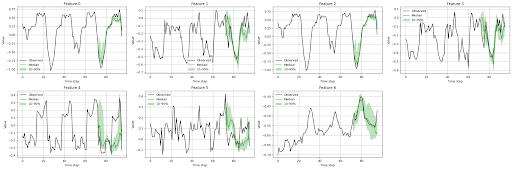
\includegraphics[width=1.0\textwidth]{figures/forecast_etth.png}}
    \caption{FITS forecast sample on ETTh time series}
    \label{fig:forecast_etth}
\end{figure}

\begin{figure}[htb]
    \centering
    \fbox{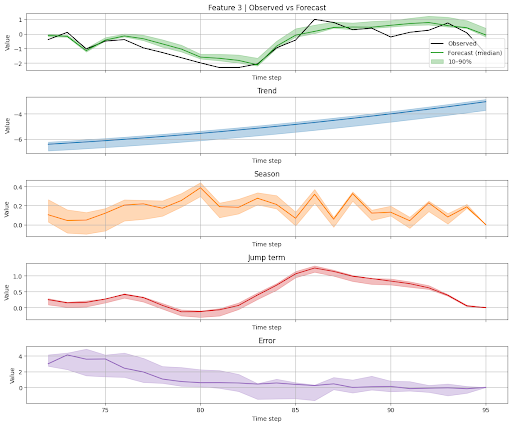
\includegraphics[width=1.0\textwidth]{figures/interpret_solar.png}}
    \caption{FITS decomposition of forecast on Solar Energy time series}
    \label{fig:interpret_solar}
\end{figure}

Time-series imputation results (forecasting) is depicted on ~\ref{fig:forecast_etth}, while detailed decomposition components are depicted on ~\ref{fig:interpret_solar}.

As a result it appears that making data stationary alone makes the task of forecasting significantly easier (and even has greater effect that conditional learning), while jump component while not only adding more interpretability to the results, makes better forecasting itself while not making model significantly heavier.
